% Created 2020-04-23 Thu 18:11
% Intended LaTeX compiler: pdflatex
\documentclass[11pt]{article}


%%%%%%%%%%%%%%%%%%%%%%%%%%%%%%%%%%
% PACKAGES
%%%%%%%%%%%%%%%%%%%%%%%%%%%%%%%%%%
\usepackage[utf8]{inputenc}
\usepackage[T1]{fontenc}
\usepackage{grffile}
\usepackage{longtable}
\usepackage{wrapfig}
\usepackage{rotating}
\usepackage[normalem]{ulem}
\usepackage{textcomp}
\usepackage{capt-of}

\usepackage{multicol} % multiple columns
\usepackage{fancyhdr} % page number in bottom right
\usepackage{graphicx} % images
\usepackage{float} % float image in columns, gives [H]
\usepackage{amsmath, amssymb} % maths symbols / environments

\usepackage{geometry} % Page Margins
\usepackage{hyperref} % PDF metadata setup.
% \usepackage{mathptmx} % Use times font face for maths
\usepackage{caption} % Tighter caption control.

\usepackage{csquotes} % quotation

\usepackage{listings} % code listing

%%
% syntax highlight
%%
\usepackage{color} 

\definecolor{dkgreen}{rgb}{0,0.6,0}
\definecolor{gray}{rgb}{0.5,0.5,0.5}
\definecolor{mauve}{rgb}{0.58,0,0.82}

\lstset{frame=tb,
  language=C++,
  aboveskip=3mm,
  belowskip=3mm,
  showstringspaces=false,
  columns=flexible,
  basicstyle={\small\ttfamily},
  numbers=none,
  captionpos=b,
  numberstyle=\tiny\color{gray},
  keywordstyle=\color{blue},
  commentstyle=\color{dkgreen},
  stringstyle=\color{mauve},
  breaklines=true,
  breakatwhitespace=true,
  tabsize=3
}


%%%%%%%%%%%%%%%%%%%%%%%%%%%%%%%%%%
% FORMATTING REQUIREMENTS
%%%%%%%%%%%%%%%%%%%%%%%%%%%%%%%%%%
\geometry{top=2.5cm, bottom=2.5cm, left=2cm, right=2cm}
\linespread{1.05} % 1.05x line spacing.
\setlength{\columnsep}{0.7cm} % 0.7cm column spacing.
\setlength{\multicolsep}{0cm}
\setlength{\parskip}{6pt} % 6pt skip between paragraphs
\setlength{\parindent}{0pt}
\newcommand{\figsquish}{\vspace{-5mm}} % Hack to fix poor figure spacing due to [H]

% Captions
% Table captions go above, 6pt space, small (9pt) roman font, roman numeral counting.
\captionsetup[table]{position=above, skip=6pt, font={small, rm}}
\renewcommand\thetable{\Roman{table}}
% Figure captions go below, 5pt space, small (9pt) roman font.
\captionsetup[figure]{position=below, skip=5pt, font={small, rm}}

%%%%%%%%%%%%%%%%%%%%%%%%%%%%%%%%%%
% SECTION REQUIREMENTS
%%%%%%%%%%%%%%%%%%%%%%%%%%%%%%%%%%
\usepackage{titlesec}
\titlelabel{\thetitle.\hspace{0.5cm}} % Dot between number and title on sections.
% Format is 10pt, so \large = 12pt, \normalsize=10pt
\titleformat*{\section}{\large\bfseries}
\titlespacing*{\section}{0cm}{4pt}{4pt} % 6pt from \parindent
\titleformat*{\subsection}{\normalsize\bfseries}
\titlespacing*{\subsection}{0cm}{0pt}{0pt} % 6pt from \parindent

% Set up footer.
\pagestyle{fancy}
\fancyhf{}
\renewcommand{\headrulewidth}{0pt}
\rfoot{\thepage} % page number, bottom right of page
\author{danny}
\date{\today}

% This info is reused in places, so input it here and it will be updated globally.
\newcommand{\docTitle}{Report: P20 whiteboard chat app}
\newcommand{\docAuthor}{Danny He\\Dimitrios Gkioulis}

\hypersetup{
 pdfauthor={danny},
 pdftitle={Report: P20 whiteboard chat app},
 pdfkeywords={},
 pdfsubject={},
 pdfcreator={Emacs 26.3 (Org mode 9.1.9)}, 
 pdflang={English}}

%%%%%%%%%%%%%%%%%%%%%%%%%%%%%%%%%%
% DOCUMENT BEGIN
%%%%%%%%%%%%%%%%%%%%%%%%%%%%%%%%%%

\begin{document}
{
    \centering
    % Use size 28 font. 1.05x gives 29.4pt line spacing.
    \fontsize{28pt}{29.4pt} \selectfont
    \docTitle\\
    \vspace{25pt}
    % Name block.
    %% \fontsize{11pt}{11.55pt}\selectfont
    %% \docAuthor\\
    \fontsize{10pt}{10.5pt}\selectfont
    {Danny He} \textit{dyh1g19@soton.ac.uk} \\ % add your email address
    %% \textit{Personal Tutor: Dr Soon X Ng} \\ % add your personal tutor
    {Dimitrios Gkioulis} \textit{dg2u19@soton.ac.uk} \\
}

\tableofcontents

\newpage

\begin{multicols*}{2}
\section{Background}

\subsection{Read up on threads and mutexes}

Threading is a technique used to enable software level parallism. Multi-core is similar to multi-threading in the sense of multi-tasking and parallism, but in hardware. A single-core CPU can still have some level multi-tasking, by saving current states of execution and load a saved state of another program for its execution.

Using threads means the danger of introducing race-conditon into the equation. This also refers back to when we leant interrupts in elec1200, where current execution halts and execute the code in the interrupts, this will be an issue if the instruction, which the program halts at was a 16-bit one, was updating data that is shared with the interrupts.

This issue can be resolved by using mutex with care. Avoid casuing deadlocks and other issues while making the program thread-safe.

\section{Implementation}

\subsection{The GUI send and receive windows + Project general structure}

% talk about structure of the project fig:draw-win-design

% project modularity
My drawing window are designed in a way that they can both transmit and receive drawings from each other, this can be achieved by using a bi-directional communication class, that bridges between two windows.

\begin{figure}[H]
  \centering
  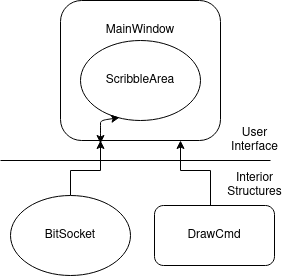
\includegraphics[width=0.75\columnwidth]{draw-win-design}
  \caption{draw window design}
  \label{fig:draw-win-design}
\end{figure}
\figsquish

My project will follow a construct show in figure~\ref{fig:draw-win-design}, %% ``bitSocket'' is an actual class implemented for a later class. However, the idea of modularity still holds here. If it was whatever feature we wanted for our program to have network-wise, the only module(class) that will be affected is our socket class implementation. It would still provides if not the same send and receive methods interfacing, at least minimal changes will be required to apply these new changes to Socket class.

%% For example, although this assignments had not specify the need for wireless connection between the clients, it can be done at later by modifying the Socket class again

% scribble mode
The drawing windows are designed to be capable of numerous shapes outlined in code ``\nameref{lst:scribble-mode-enum}'', they are showcased in figure ``\nameref{fig:showcase_drawCmd}''.

\begin{lstlisting}[label=lst:scribble-mode-enum, caption={ScribbleMode enum}]
enum ScribbleMode
{
    cursor = 1, // disable custom draw event
    undo,
    //
    raw_line, // draw line from each mouse move
    smooth_line, // draw raw_line, but replace it with smooth line
    straight_line, // draw a line from start to end
    circle,
    rectangle,
    //
};
\end{lstlisting}

% How will the send-window allow users to draw diagrams?
My \verb|scribbleArea| class that is the core of the draw window, utilizes \verb|QGraphicsView| to render drawings. Mouse events are captured to `draw' the shapes, in order to capture these events: pressed; move; released, I had to apply an \verb|eventFilter| on \verb|QGraphicsView|. Besides \verb|raw_line|, which is continuously drawing small segment of lines, all other shapes are to be updated to the mouse point and only drawn until mosue release.

% undo -> painter classes used for scribbleArea
I also wanted to implement \verb|undo|, which will be a very useful feature. It was fairly trivial to implement because I used \verb|QGraphicsView| with \verb|QGraphicsScene| for my ScribbleArea. All drawing objects that I added to \verb|QGraphicsScene| are subclassed of \verb|QGraphicsItem|. I can use \verb|removeItem| on \verb|QGraphicsScene| to remove any of those items, and I keep track of all the items drawn with a vector. 

\begin{figure}[H]
  \centering
  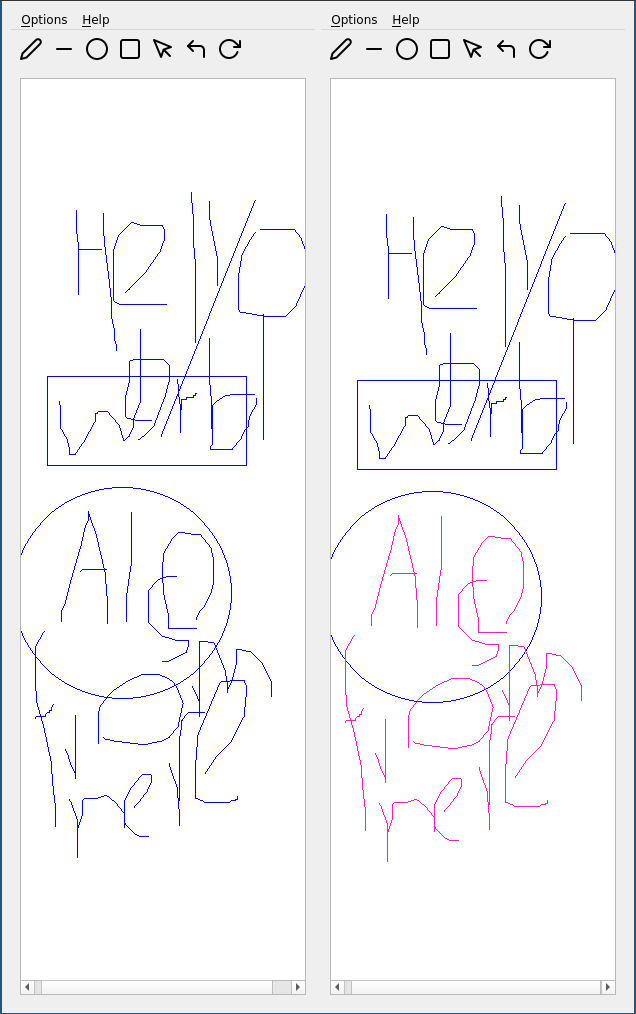
\includegraphics[width=\columnwidth]{show_all_draw}
  \caption{showcasing all the drawing commands}
  \label{fig:showcase_drawCmd}
\end{figure}
\figsquish

The figure above (figure~\ref{fig:showcase_drawCmd}) showcases all of the available shapes for drawing.

\subsection{Serialize and deserialize drawing-commands}

\subsubsection{serialize commands}

% Drawing command repreentaiton
Looking at the struct \verb|ScribbleMode| at code~\ref{lst:scribble-mode-enum}.
Cursor and undo are special commands, i.e they are not drawing commands.
Cursor is very special in that sense, because it's the only mode that will not be transmited mouse movement data.
Undo is the only commands that has no other information transmitted.
The most important modes are the lines, circle and rectangle.
In our choosen way of representing the drawing board. Besides the \verb|raw_line| raw\_line mode, all the rest of the modes (\verb|straight_line|, \verb|circle|, \verb|rectangle|), can have their shape defined with two points. This is very handy, because now we can define an unform interface/data-structure to represent it:

\begin{lstlisting}[caption={DrawCmd struct}]
struct DrawCmd {
    uint mode;
    QPointF p1;
    QPointF p2;
}

struct QPointF {
    // a pseudo implementation for demonstration purposes
    qreal x;
    qreal y;
    ...
}
\end{lstlisting}

Note that QPointF is a type part of the Qt framework, the implementation here is to illustrated its interior structure for the serialization process, it may not be the actual implementation.

\begin{lstlisting}[label=lst:deserialization-sequence, caption={How DrawCmd will be structured put into a struct}]
struct toBeSerialized {
    uint mode,
    qreal x1;
    qreal y1;
    qreal x2;
    qreal y2;
}
\end{lstlisting}

% serialization process
Each \verb|DrawCmd| will be serialized in the sequence of bytes as shown in the snippet above. And deserialized in a similar way.
\verb|uint| is of size 1 byte. 'qreal' is a Qt type which can be double or float, by default it is double. It's size doesn't not matter too much, because we can use sizeof operator to determine the actual size in bytes. 
This design is not sustainable, however, if we want to implement feature such as moving a drawn figure, extra fields(bytes) will be required to introduced, to include information about which drawing item to be moved.

To use \verb|DrawCmd|, I implemented the following interfacing methods:

\begin{lstlisting}
struct DrawCmd {
    ...
    DrawCmd(byte_t *data) { /* deserialize */ }
    // the total size will be pass out into pointer size
    byte_t* serialize(uint *size) {  /* serialize */ }
}
\end{lstlisting}

To serialize DrawCmd, I first allocated the memory required for data using \verb|malloc|.
Then I used \verb|memcpy| to directly copy the each data into the corresponding address space without any encoding (see code listing \nameref{lst:deserialization-sequence})
Similarly, for deserialization, I use memcpy to copy from the data sequence back into each of the fields.
Finally, to help aiding the development of my serialization interface I used a Qt test library, before adding the serialization into my program.

% unit testing
\begin{lstlisting}[caption={unit testing}]
./unitTests/unitTests.pro
// new project for unit testing
QT += testlib
... // bit more stuff

./unitTests/test.cpp // unit testing implementation
void testSerialization() {
    DrawCmd cmd(QPointF(0.2, 0.3), QPointF(0.2, 0.4));
    //
    uint size = 0;
    byte_t* data = cmd.serialize(&size);

    DrawCmd deserialized = DrawCmd(data);

    // testing code ommited
    ...
    //
    free(data);
}
\end{lstlisting}

\begin{lstlisting}[caption={unit testing log, it showed all tests had passed}]
** Start testing of UnitTests *********
   Config: Using QtTest library 5.14.2, Qt 5.14.2 (x86\_64-little\_endian-lp64 shared (dynamic) release build; by GCC 9.3.0)
   PASS : UnitTests::initTestCase()
   PASS : UnitTests::vectorSerialization()
   PASS : UnitTests::serialization()
   PASS : UnitTests::cleanupTestCase()
   Totals: 4 passed, 0 failed, 0 skipped, 0 blacklisted, 0ms
** Finished testing of UnitTests *********
\end{lstlisting}

\subsubsection{use serialize for communication}

\begin{lstlisting}[label=lst:using-serialization, caption={communication code}]
void MainWindow::onNewDiagramDrawn(DrawCmd cmd)
{
    uint size = 0;
    byte_t* data = cmd.serialize(&size);
    bitsock->sendData(data, size);
    printf("sent: \n");
    //
    free(data);
}

void MainWindow::onDataReceived(Bytes_t data)
{
    DrawCmd cmd(data.data());
    printf("Receivded: \n");
    cmd.print();
    QGraphicsItem *item = this->scribbleArea->applyNewDrawCmd(cmd);
    items.push_back(item);
}
\end{lstlisting}

\begin{figure}[H]
  \centering
  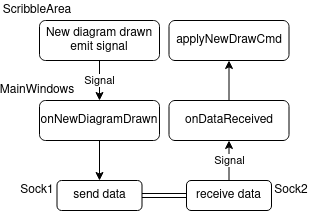
\includegraphics[width=\columnwidth]{serialize-flowchart}
  \caption{communication process}
  \label{fig:serialize-flowchart}
\end{figure}
\figsquish

The process of communication can be best described in figure~\ref{fig:serialize-flowchart}.

\begin{lstlisting}[label=lst:serialization-log, caption={serialized data pass through in communication}]
sent: {0x3 0 0 0 0 0 0 0x46 0x40 0 0 0 0 0 0x10 0x70 0xffffffc0 0 0 0 0 0 0 0x44 0x40 0 0 0 0 0 0xffffffe0 0x6f 0xffffffc0 0 0 0 0 }
Receivded: {0x3 0 0 0 0 0 0 0x46 0x40 0 0 0 0 0 0x10 0x70 0xffffffc0 0 0 0 0 0 0 0x44 0x40 0 0 0 0 0 0xffffffe0 0x6f 0xffffffc0 0 0 0 0 0 }
DrawCmd { 3 44.000000 -257.000000 40.000000 -255.000000 }
\end{lstlisting}

From the log ``\nameref{lst:serialization-log}'', we can see that there are a lot of zeros, encoding the data as in is an overkill. It also seems that the data are actually integer, but are stored in \verb|qreal|, which is of type float, for convenience sake. For optimizations, use integer type instead of qt type. and encoding them in a smaller range, i.e 2 bytes range \( \text{2 bytes} = 2^8*2 = 65536 \), which is more than sufficient for the number of pixels on our computer monitors.

\subsection{Implement send and receive threads}
   %% Implement send and receive threads, where the send thread takes serialized commands and will send these, while the receive thread will read data and pass them to the receive window. For now, just test this by passing serialized commands using a queue. You may want to implement a thread-safe queue template class to do this.

   % bring up modularity that threading will be limited to Socket class only

   % i did not need to implement threads.  
   Originally I did not need to implement threads because I used my Socket class, which is an abstration over \verb|QTcpSocket| and \verb|QTcpServer|. It uses \verb|QIODevice::readyRead| signal and emits a new signal with the deserialized \verb|DrawCmd|. The drawing windows listens to that signal and render the drawings in.

   However, later on when we are required to code our own communication protocol. It become evident that \verb|thread| will be used.

   I first began using \verb|std::thread|, when I found out it was not allowed for some reason. Fortunately, I could still use \verb|pthread|. There wasn't much change required, except \verb|pthread| is a \verb|c| threading library, it doesn't support lambda like \verb|std::thread| does. This means I couldn't pass in the lambda that captures \verb|this|, instead I need to interface it with a static class method, which takes a \verb|this| pointer, which will be passed in from \verb|pthread_create| (see BitSocket.hpp). I personally do not like this at all, because a static class method had to be put into the header file. Having all the code within the same \verb|cpp| file is much easier to navigate.

   The receive thread function, is illustrated by the following pseudocode:
\begin{lstlisting}[caption={receive thread function pseudocode}]
  while (true) {
    get data from gpio // this block, only return if there is any data received
    emit the data received signal with the data
  }
\end{lstlisting}

   For sending I did not use thread. As I did not experience any lag while drawing in my application, I understand this is may be because I am testing on my own computer, the connection is local. For this program to work perhaps with more than two connections, and wirelessly, I intended to use \verb|thread| with a sending queue.

\begin{lstlisting}[caption={}]
  // thread function
  while (true) {
    get mutex queue // will be block if queue is accessed else where
    if queue not empty {
      pop queue
      send popped data
    }
  }
  // my socket class send function
  get mutex queue // will be block if queue is accessed else where
  add sending data to queue
\end{lstlisting}

   
\subsection{Implement your communication protocol using booleans}
\label{sec:comm-protocols}
In your report, you are expected to explain how your communication protocol works, for example detailing what signalling you are implementing between the send and receive windows and how data is exchanged. In the report, you can illustrate your code using pseudocodes or flowcharts. 

Implement and test your bit-stream communication protocol, by toggling shared Boolean variables, which are emulating the role of GPIO pins if you are communicating between two different Pis. Remember you need to think about how to signal when a bit is ready to read, and when it has been read.  Hint: You may need to use mutexes to avoid race conditions.

\begin{figure}[H]
  \centering
  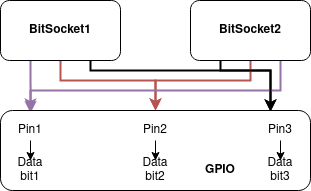
\includegraphics[width=0.7\columnwidth]{gpio-design}
  \caption{gpio simulator diagram}
  \label{fig:gpio-design}
\end{figure}
\figsquish

For this part, I decided to simulate GPIOs that are ony the raspberry pi. Firstly, the coursework was originally designed to communitate via the GPIO pins. Secondly, the bit-stream and shared boolean for the communication protocol, making a GPIO class seems to be a perfect fit.

\begin{lstlisting}[caption={GPio class illustration}]
  // ./gpio/gpio.hpp
  class GPio {
    static GPio* getInstance() { ... }
    void setPinTo(uint pinNum, bit_t bit) { ... }
    bit_t getPin(uint pinNum) { ... }
  }
\end{lstlisting}

Each pin number corresponds to a mutexed \verb|bit_t| number (typedef bool \verb|bit_t|). GPio class keep track of all the pins with a vector, and populate it with a \verb|mutex<bit_t>|. The getter and setter methods of \verb|GPio| actually doesn't call lock or unlock at all, instead the mutex class I used, is my custom mutex class, that is a wrapper of std::mutex, which can hold data while function as mutexes, takes care of the lock and unlock in the get and set methods. However, that would only work for data that aren't of more complex structure, I implmented \verb|getRef|, \verb|lock| and \verb|unlock| for that purpose.

\begin{lstlisting}[caption={my mutex class illustration}]
// ./gpio/mutex.hpp
class mutex
{
public:
    mutex() {}
    mutex(T defaultVal) { ... }
    // gettors
    T get() { ... }
    void set(T x) { ...}
    //
    T& getRef() { ... }
    void lock() { m.lock(); }
    void unlock() { m.unlock(); }
private:
    std::mutex m;
    T data;
}
\end{lstlisting}

In each of the interfacing methods of \verb|mutex|, \verb|lock| and \verb|unlock| are called onto the \verb|mutex m| before performing the accessing or setting procedure.

% BitSocket bit-stream implementation
Finally, with all the infracstructure in place.

\begin{lstlisting}[caption={BitSocket class illustration}]
// ./gui-bit-stream/BitSocket.hpp
class BitSocket
{
public:
    void sendData(const char *data, uint size);
    QVector<char> recvData(uint size);
signals:
    void dataReceived(Bytes_t data);
private:
    // more field ommited
    int txDataPin = -1; // send data pin channel
    int txFlagPin = -1;
    int txLockPin = -1;
    //
    int rxDataPin = -1;
    int rxFlagPin = -1;
    int rxLockPin = -1;
    //
    void sendByte(char abyte);
    char readByte();
}
\end{lstlisting}

BitSocket uses 6 pins in total, 3 pins each for receiving and sending data. It is bidirectional. The lockPins were originally thought of to prevent race-condition when multiple sends are called, but that won't happen because send methods right now will only be called sequencetially. Instead it serves the purpose to prevent deadlock in \verb|readByte| that \verb|recvData| uses. It also works similar to UART, where rx pins will need to be connected to the tx pins at the other end of the connection.

% explain communication protocol
\begin{figure}[H]
  \centering
  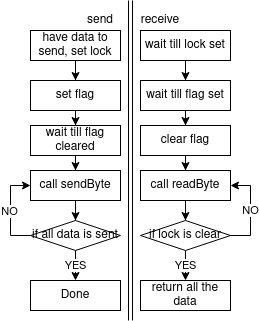
\includegraphics[width=0.75\columnwidth]{communication-protocol}
  \caption{communication protocol illustration}
  \label{fig:communication-protocol}
\end{figure}
\figsquish

\begin{lstlisting}[caption={BitSocket class methods illustration}]
void BitSocket::sendByte(char abyte) {
  loop 8 times {
    get the most significant bit
    set data pin to that bit
    set flag pin to 1
    loop until flag pin is set to 0 // make sure data is read
    cycle new bits with << operator
  }
}

char BitSocket::readByte() {
  loop until flag pin is set to 1 // make sure data is read
  loop 8 times {
    bit <- read data pin
    abyte <- collect read bit
    clear flag pin // inform bit read
  }
  return abyte
}
\end{lstlisting}

% draw them on the receive window
listing ``\nameref{lst:serialization-log}''
After receiving the serialized data bytes in the following form (quotation below). It is just called the deserialization constructor as shown in ``\nameref{lst:using-serialization}''.

\begin{displayquote}
\{0x3 0 0 0 0 0 0 0x46 0x40 0 0 0 0 0 0x10 0x70 0xffffffc0 0 0 0 0 0 0 0x44 0x40 0 0 0 0 0 0xffffffe0 0x6f 0xffffffc0 0 0 0 0 \}
\end{displayquote}

The final result is shown in figure~\ref{fig:showcase_drawCmd}, besides showcasing all of the drawing commands, it is also complete product.

\section{Bug fixes \& Enhancements}

\subsection{Implement send threading and queue}

Later during the testing of the program, I notices lag on undoing lots of raw lines drawn, or clearing the drawing, that had lots drawn, will block the ui. To resolve this, I came to my senses and decided to implement a threaded send queue.

\begin{lstlisting}[label={lst:new-thread-worker-fn}, caption={new thread worker fn}]
  while (true) {
    bool sent = false;
    if (self->hasDataToRecv()) {
      // arbitrary number 64 used
      // but 32 bytes at least
      auto data = self->recvData(64);
      self->dataReceived(data); // emit signal
    }
    while (self->hasDataToSend()) {
      if (!sent) sent = true;
      self->sendQueuedData();
    }
    if (!sent) nanosleep(self->tim, NULL);
  }
\end{lstlisting}

From ``\nameref{lst:new-thread-worker-fn}'', we crammed both the send and recieved in the thread-fn. While this seem like a perfect solution to the problem addressed earlier, I realized after some thoughts: this might cause deadlock, i.e if both user are to drawing at an incredible speed, faster or similar to the speed that the data are transmitted, or if they are simply drawing at the same time, first user will be stuck in the send loop, while sending. After the other user finishes receiving the data, they will proceed to be stuck in the send loop as well, because both users are sending, none receiving.
This could be fixed by fixing the outlier mechanics of \verb|raw_line|, the only draw mode that continuously draw. It can be changed so it behave the same as the rest, only fixated itself after mouse release. Given the fastest drawn event will be a tap, the world records state the fastest click time for 10 seconds is 1,051 times. Roughly 100 clicks per second, 0.1 clicks per millisecond. So sending 1 drawCmd every 10 millisecond, that would be enough time for thread loop to continuously looping to prevent deadlock.

\subsection{Make your communication protocol more robust}

Yet another during the a later time, testing the functionality of my program. I noticed clearing the draw window will not clear all drawings on the other users' side, there will always be some left overs.

Looking at the logs, after adding some debug outputs:

\begin{lstlisting}[caption={output log with error}]
flag cleared while reading ERROR
...
Received: {0x2 0 0 0 0 0 0 0 0 0 0 0 0 0 0 0 0 0 0 0 0 0 0 0 0 0 0 0 0 0 0 0 0 0 0 0 0 0 0x12 0xffffff81 0 0 0 0 0 0 0 0 0 0 0 0 0 0 0 0 0 0 0 0 0 0 0 0 0 0 0 0 0 0 0 0 0 0 0 0 0x9 0x40 0xffffff80 0 0 0 0 0 0 0 0 0 0 0 0 0 0 0 0 0 0 0 0 0 0 0 0 0 0 0 0 0 0 0 0 0 0 0 0x4 0xffffffa0 0x40 0 0 0 0 0 0 0 0 0 0 0 0 0 0 0 0 0 0 0 0 0 0 0 0 0 0 0 0 0 0 0 0 0 0 0 0x2}
\end{lstlisting}

\begin{lstlisting}[caption={Correct output log}]
Received: {0x2 0 0 0 0 0 0 0 0 0 0 0 0 0 0 0 0 0 0 0 0 0 0 0 0 0 0 0 0 0 0 0 0 0 0 0 0 }
DrawCmd { 2 0.000000 0.000000 0.000000 0.000000 }
\end{lstlisting}

The above log shows The correct and successfull transmission, while the one above that is the part of the logging during a clear.

From the logs, it seems to me that the sending is way too frequent, which somehow the receive end captures way too many packets while it is meant to receive one only.

At the time I made some changes to the protocol, recall in the original protocol shown in figure~\ref{fig:communication-protocol}, the receive end decides to stop receiving bytes until the \verb|lockFlag| is set. I changed it so, the send end will send the number of bytes in this packet, before sending. The receive end will read the packet size before reading(receiving) each bytes in the packets. This change in logic, removes the worrying of the receiving end not knowing how many bytes it should receive, which I actually had a bit more code at the end of the receive data function to check for the \verb|lockFlag| to see if more data should be received, essentially a double receive to compensate for that worry in my mind. Now this extra bit is removed because of the change in protocol outlined just now. After that the program clears drawing as expected.

%%%%%%%%%%%%%%%%%%%%%%%%%%%%%%%%%%
% End
%%%%%%%%%%%%%%%%%%%%%%%%%%%%%%%%%%
\end{multicols*}
\end{document}